\begin{frame}{\ptthreeofour surface reconstructions}
    \begin{columns}
    
    \column[T]{0.38\textwidth}

    \begin{overprint}
        \onslide<1>\begin{table}
        % \begin{table}
            \centering
            \begin{tabular}{ |l|l|l|l| }
                \hline
                Argon & \ammonia & \dioxygen & Duration \\
                 & & & (hours) \\ 
                \hline
                50 & 0 & 0 & 24 \\
                42 & 0 & 8 & \cellcolor{Important} 12 \\
                41 & 1 & 8 & 5 \\
                \hline
                50 & 0 & 0 & 7 \\
                42 & 0 & 8 & \cellcolor{Important} 1 \\
                \rowcolor{shadecolor}
                41 & 1 & 8 & 10 \\
                48.5 & 1 & 0.5 & 13 \\
                49 & 1 & 0 & 11 \\
                50 & 0 & 0 & 8 \\
                \hline
            \end{tabular}
            \caption{Gas flow in reactor ($50$ mL/min, $0.3$ bar). In experimental order.}
        \end{table}
        \onslide<2>\begin{figure}
            \centering
            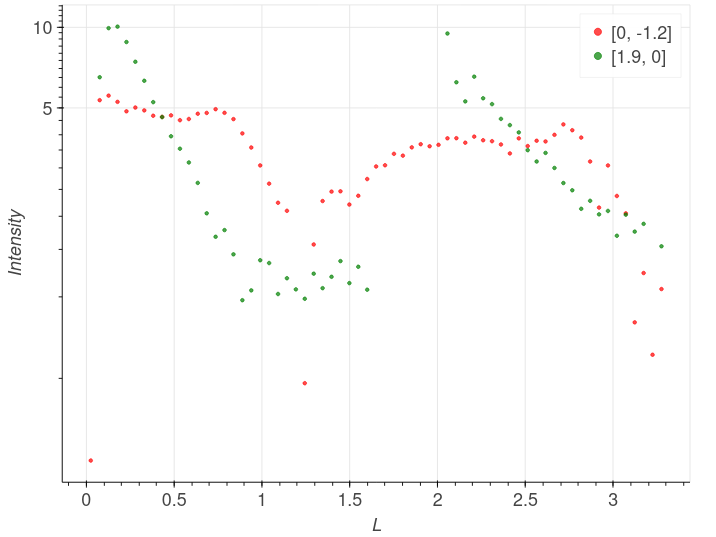
\includegraphics[width=0.95\textwidth]{Figures/sxrd_data/ctr/reconstruction_ctr_condE.png}
            \caption{CTR, peaks at L={0.7, 1.4, 2.1, 2.8} are characteristic of \ptthreeofour (red dots). The background shape is linked to xxx. The peaks for the green dots are linked to xxx.}
            \label{fig:ctr_conde}
        \end{figure}
    \end{overprint}

    % add fit with ROD

    %\vspace{-0.5cm}

    The second structure does not disappear this time when adding \ammonia. Instead we have $10\times10$ reconstructions for \ptthreeofour.

    \column[T]{0.6\textwidth}

    \begin{figure}
        \centering
        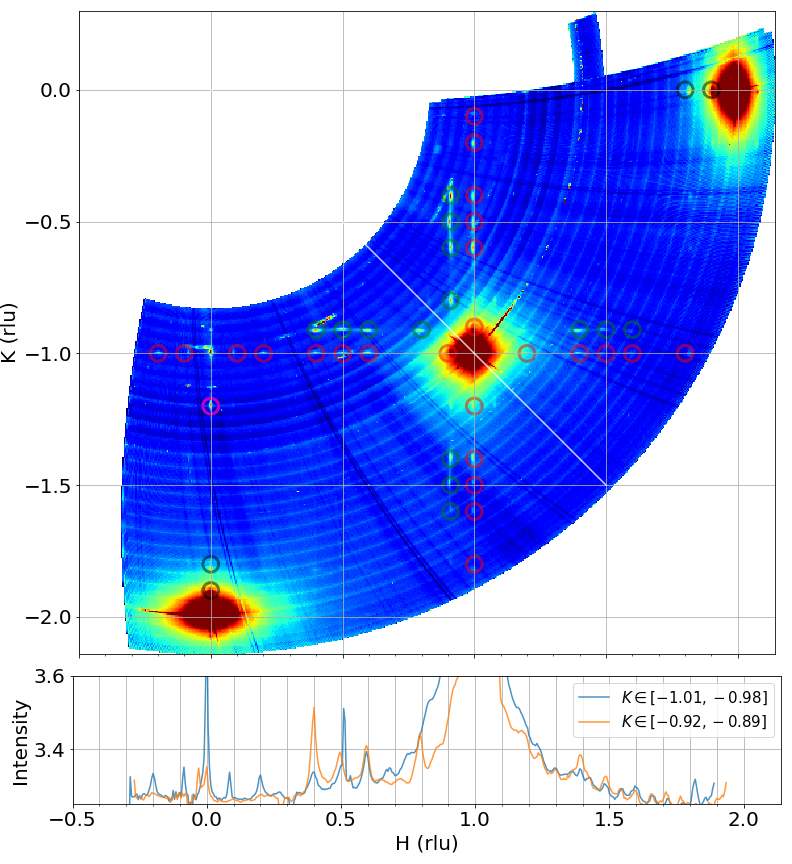
\includegraphics[width=0.79\textwidth]{Figures/sxrd_data/maps/band_in_k_reconstructions.png}
        \caption{Reciprocal space in-plane map under reacting conditions (top), map integration highlighting reconstruction peaks (bottom).}
        \label{fig:CondE2}
    \end{figure}
    \end{columns}
    
\end{frame}